\section{Prvočísla -- popište způsob generování a~uveďte příklad pravděpodobnostního testu a~skutečného testu}

Jsou extrémně důležitá pro téměř všechny kryptosystémy: asymetrické šifrování, digitální podpisy, ustanovení klíčů i~vyšší systémy (TLS, PKI).

Prvočísel je nekonečně mnoho, počet $\pi(n)$ menší než $n$ lze pro~velké hodnoty aproximovat jako $\pi(n) = \frac{n}{\ln(n)}$. Současné kryptosystémy využívají prvočísla o~velikosti 2048-4096b (600 - 1200 cifer).

\subsection{Typy prvočísel}

\textbf{Mersennova prvočísla}: $M_p = 2^n - 1$ (např. 31). \\
\textbf{Sophie-Germain prvočísla}: $p$ pokud $2p + 1$ je také prvočíslo (např. 11). \\
\textbf{Bezpečná prvočísla}: $B_p = 2p + 1$ (např. 23). Jsou generována SG prvočísly.

\subsection{Generování}

Velmi neefektivním způsobem je Eratosthenovo síto. Sestaví se seznam všech čísel od~2 do~$n$. První se ze~seznamu vyřadí a~prohlásí se za~prvočíslo, všechny jeho násobky se ze~seznamu vyřadí. Takto se pokračuje dokud nedosáhneme $\sqrt{n}$, kdy zbývají pouze prvočísla.

Prakticky se buď volí bezpečná prvočísla, nebo se náhodně vygeneruje číslo požadované velikosti a~otestuje se, zda se o~prvočíslo jedná.

\subsection{Pravděpodobnostní testy}

\textbf{Fermatův test} je založen na~modulárním mocnění. Zvolíme libovolné $a: 1 \leq a \leq n-1$, spočteme $a^{n-1} \stackrel{?}{\equiv} 1 \Pmod n$. Pokud kongruence platí, opakujeme pro~jiné $a$, pokud neplatí, $n$ prvočíslo není. Čím více pokusů, tím větší šance že se o~prvočíslo jedná. Nedokáže odlišit prvočísla a~Carmichaelova čísla\footnote{%
Carmichaelovo číslo splnňuje kongurenci $b^{n-1} \equiv 1 \Pmod n$ pro~všechna $b$ nesoudělná s~$n$.
}.

\noindent \textbf{Miller-Rabinův test} je spolehlivější než~Fermatův; složená čísla projdou iterací s~maximálně 25\% pravděpodobností.

\begin{table}[ht]
\begin{tabular}{l|l}
0 & $n = 2^s r + 1$ kde $r$ je liché \\
1 & $a: 1 \leq a \leq n-1$ \\
2 & $\begin{cases}
a^r \equiv 1 \Pmod n & \mathrm{nov\acute{a}\ iterace} \\
a^r \not\equiv 1 \Pmod n & \mathrm{bod\ 3} \\
\end{cases}$ \\
3 & Platí $a^{2^i r} \equiv n-1 \Pmod n$ pro všechna $i: 0 \leq i \leq s-1$ $\begin{cases}
\mathrm{ano:} & \mathrm{nov\acute{a}\ iterace} \\
\mathrm{ne:} & \mathrm{je\ slo\check{z}en\acute{e}} \\
\end{cases}$ \\
\end{tabular}
\end{table}

\subsection{Skutečné testy}

\textbf{Lucas-Lehmerův test} funguje pouze pro~Mersenova prvočísla ($M_p = 2^s - 1$). \\
$u_0 = 4$, $u_{n+1} = (u_n^2 - 2) \Mod n$, \dots, $u_{s-2} \stackrel{?}{=} 0$.

\clearpage
\section{Teorie čísel, algebraické struktury -- popište účel a~způsob výpočtu Eulerovy funkce. Popište požadavky na grupu a způsob generování grupy pro algoritmy založené na problému DL.}

Teorie čísel je část matematiky zkoumající vlastnosti (zejména) celých čísel. Prvočíslo je $p \geq 2$, které nemá jiné dělitele než triviální. Každé celé číslo $\geq 2$ je buď prvočíslo nebo se dá zapsat jako součin prvočísel. Pokud číslo není prvočíslo, nazýváme ho číslem složeným.

V kryptografii se nejčastěji setkáme s dělitelností (zbytek a~modulo), největším společným dělitelem (GCD, výpočet jako násobek společných prvočinitelů s~jejich nejmenší mocninou), nejmenším společným násobkem (LCM, výpočet jako násobek všech prvočinitelů s~největší mocninou). Jestliže jsou výsledek GCD roven 1, jedná se číslo nesoudělné a~bude se nejspíše jednat o~prvočíslo.

\textbf{Eulerova funkce} $\phi(n)$ je často používaná v~kryptografii. Udává počet celých čísel, která jsou nesoudělná s~$n$.

\begin{table}[ht]
    \centering
    \caption{Výpočet Eulerovy funkce $\phi$}
    \begin{tabular}{l|l}
        prvočísla & $\phi(n) = n-1$ \\
        mocniny prvočísel & $\phi(p^k) = (p-1) p^{k-1}$ \\
        složená čísla & $\phi(a \cdot b) = \phi(a) \cdot \phi(b)$ \\
    \end{tabular}
\end{table}

Algebraické struktury představují množiny prvků s~operacemi a~různými vlastnostmi. V~kryptografii jsou nejpoužívanější grupy, tělesa a~konečná tělesa.

\textbf{Grupou} (G, $\circ$) nazýváme množinu G spolu s binární operací $\circ$ (operace se dvěma prvky $a, b$ kterým přiřazuje prvek $c$ stejné grupy) na~množině G, která splňuje:

\begin{itemize}[noitemsep]
    \item uzavřenost (pro všechny prvky $a, b$ v~G je i~$a \circ b$ prvkem G)
    \item asociativita $(a \circ b) \circ c = a \circ (b \circ c)$
    \item existence neutrálního prvku (existuje prvek e v G takový že pro všechna $a$ v~G platí $a \circ e = e \circ a = a$)
    \item existence inverzního prvku (pro každý prvek $a$ existuje prvek $b$ takový že $a \circ b = b \circ a = e$, tj. že jejich složení je rovno neutrálnímu prvku. Prvku $b$ se říká inverzní)
\end{itemize}

Grupa (G, $\circ$) je \textbf{cyklická}, jestliže existuje prvek $a$ v~G takový, že pro každé $b$ v~G existuje celé číslo $i$ takové, že $b = a^i$. Takový prvek se nazývá generátor grupy. 

Řád prvku $a$ je definován jako nejmenší kladné celé číslo $t$ takové že $a^t = 1$ pokud takové $t$ existuje. 

Řád generátoru grupy se rovná řádu grupy. Počet generátorů lze zjistit jako $\phi(\phi(n))$.

Příklady praktických grup pro~kryptografii:
\begin{itemize}[noitemsep]
    \item Množina celých čísel $\mathbb{Z}$ spolu s operací sčítání (+) tvoří abelovskou grupu.
    \item Množina $\mathbb{Z}_n$ s operací sčítání modulo $n$ tvoří grupu řádu $n$.
    \item Množina $\mathbb{Z}_n$ s operací násobení modulo $n$ ($\mathbb{Z}_n^*$) netvoří grupu, protože inverzní prvek neexistuje ke všem prvkům ze $\mathbb{Z}_n$.
    \item Množina $\mathbb{Z}_p$ s operací násobení modulo prvočíslo $p$ tvoří grupu, protože inverzní prvek existuje ke všem prvkům ze $\mathbb{Z}_p$. 
\end{itemize}

Příklad pro $\mathbb{Z}^*_{17}$:
\begin{itemize}[noitemsep]
    \item Grupa obsahuje prvky 1--16 celkem $\phi(17) = 16$.
    \item Neutrální prvek je $e = 1$.
    \item Každý prvek $a$ má inverzní prvek $a^{-1}$, protože pro~každé $a$ platí GCD($a$,17) = 1.
    \item Generátorem grupy jsou čísla $3,5,6,7,10,11,12,14$ a celkem je jich $\phi(16) = 8$
\end{itemize}

Nalezení generátoru:
\begin{itemize}[noitemsep]
    \item Zvolení náhodného prvku $g$ z $\mathbb{Z}_n^*$.
    \item Výpočet $\phi(n)$.
    \item Nalezení všech prvočíselných dělitelů $\phi(n)$ označených jako $p_i$.
    \item Pro každého prvočíselného dělitele se vypočte $g^{\phi(n)/p_i} \equiv 1 \mod n$.
    \item Pokud předchozí rovnice neplatí pro žádné $p_i$ jedná se generátor.
\end{itemize}

\clearpage
\section{Modulární aritmetika -- popište algoritmus Square and Multiply a Čínskou větu o zbytcích.}

Modulární aritmetika pracuje s~celými čísly v~daném intervalu. Pro~čísla platí: \\
-- \textbf{reflexivita}: $a \equiv a \Pmod n$ \\
-- \textbf{symetrie}: $a \equiv b \wedge b \equiv a \Pmod n$ \\
-- \textbf{tranzitivita}: $a \equiv b \wedge b \equiv c \Rightarrow a \equiv c \Pmod n$

\vspace*{1em} \noindent
\textbf{Malá Fermatova věta} urychluje modulární mocnění: \\
$a^p \equiv a \Pmod p$ (také \enquote{$a^p - a$ je dělitelné $p$}).

\vspace*{1em} \noindent
\textbf{Eulerova-Fermatova věta} umožňuje získat inverzní prvek: \\
$a^{-1} = a^{\phi(n) - 1} \Mod n$. Obecně platí $a^{\phi(n)} = 1 \Mod n$

\vspace*{1em} \noindent
\textbf{Rozšířený Euklidův algoritmus} umožňuje získat inverzní prvek (zde $5^{-1} \Mod 12$):

\begin{table}[ht]
	\centering
\begin{tabular}{ll|l}
	$12 = n$                               & {}                                           & \boxed{\stackrel{?}{\pm} 5} $=$ {\color{violet}2} $\cdot$ {\color{blue}2} + {\color{brown}1} (mod 12) \\
	\hline
	$5 = x$                                & {\color{violet}2} $= \lfloor 12 / 5 \rfloor$ & {\color{blue}2} = {\color{red}2} $\cdot$ {\color{brown}1} + {\color{teal}0} \\
	$2 = 12 - (5 \cdot {\color{violet}2})$ & {\color{red}2}    $= \lfloor 5 / 2 \rfloor$  & {\color{brown}1} \\
	$1 = 5 - (2 \cdot {\color{red}2})$     & {\color{purple}2} $= \lfloor 2 / 1 \rfloor$  & {\color{teal}0} \\
	$0 = 2 - (1 \cdot {\color{purple}2})$  & {}                                           & {}
\end{tabular}
\caption*{Ukázka výpočtu inverzního prvku použitím Rozšířeného Euklidova algoritmu.}
\end{table}

\noindent
Počítání probíhá nejprve v~prvních dvou sloupcích, poté zespoda nahoru ve~třetím. Po~získání výsledku je~nutné zkontrolovat znaménko (tj. je možné, že bude nutné výsledku přidat mínus a~přičíst $n$).

\subsection{Square \& Multiply}

Urychlení modulárního mocnění příkladů typu \enquote{ $a^k \Mod p$}. Při~řešení příkladu \enquote{$5^{11} \Mod 17$} lze exponent přepsat do~binární podoby: $11_{10} = 1011_2$. Jednotlivé bity se vypíší do~sloupečku tabulky odspoda nahoru (na~prvním řádku je LSB). Postupuje se zeshora dolů, a~pokud platí $k_i = 1$, vykoná se krok $b$.

\begin{table}[ht]
\centering
\begin{tabular}{c|ll}
$k_i$      & $A$                                                & $b = {\color{magenta}1}$ \\
\hline
\textbf{1} & ${\color{red}5} = a$                               & ${\color{teal}5} = {\color{magenta}1} \cdot {\color{red}5}$ \\
\textbf{1} & ${\color{violet}8} = {\color{red}5}^2 \Mod 17$     & ${\color{blue}6} = {\color{teal}5} \cdot {\color{violet}8} \Mod 17$ \\
        0  & ${\color{purple}13} = {\color{violet}8}^2 \Mod 17$ & \\
\textbf{1} & ${\color{brown}16} = {\color{purple}13}^2 \Mod 17$ & $\boxed{11} = {\color{blue}6} \cdot {\color{brown}16} \Mod 17$ \\
\end{tabular}
\caption*{Ukázka výpočtu pomocí Square \& Multiply.}
\end{table} 

\clearpage
\subsection{Čínská věta o~zbytcích}

Používá se pro~řešení soustav rovnic v~modulární aritmetice. $m_1, \dots, m_k$ jsou nesoudělná čísla. $a_1, \dots, a_k \in \mathbb{Z}$. Systém

\begin{align*}
x &\equiv a_1 \,(\mathrm{mod}\, m_1) \\
x &\equiv a_2 \,(\mathrm{mod}\, m_2) \\
&\dots \\
x &\equiv a_k \,(\mathrm{mod}\, m_k) \\
\end{align*} %
má výsledné modulo $M = m_1 \cdot m_2 \cdots m_k$. Řešení lze vypočítat vzorcem

$$ x = \sum_{i=1}^{k} a_i N_i L_i \Mod M $$
kde $M = m_1 \cdot m_2 \cdots m_k$, $N_i = M / m_i$, $L_i = N_i^{-1} \Mod m_i$.

\begin{figure}[ht]
\centering
\begin{align*}
x &\equiv 3 \Pmod 6 (= a_1 \Pmod {m_1}) \\
x &\equiv 2 \Pmod 7 (= a_2 \Pmod {m_2}) \\
M = m_1 \cdot m_2 &= 6 \cdot 7 = 42 \\
N_1 = M / m_1 &= 42 / 6 = 7 \\
N_2 = M / m_2 &= 42 / 7 = 6 \\
L_1 = N_1^{-1} \Mod m_1 &= 7^{-1} \Mod 6 = 1 \\
L_2 = N_2^{-1} \Mod m_2 &= 6^{-1} \Mod 7 = 6 \\
x = (a_1 N_1 L_1 + a_2 N_2 L_2) \Mod M &= 3 \cdot 7 \cdot 1 + 2 \cdot 6 \cdot 6 \Mod 42 = \boxed{9} \\
\end{align*}
\vspace*{-4em}
\caption*{Ukázka výpočtu čínské věty o~zbytcích.}
\end{figure}

\clearpage
\section{Symetrická kryptografie -- proudové šifry, synchronní a asynchronní proudové šifry.}
\label{question-4}

Výhodou symetrické kryptografie je velká rychlost a~malé šíření chyb, nevýhodou nízká úroveň difuze a~náchylnost k~úmyslným falzifikacím. Symetrické šifry jsou vhodné pro~šifrování velkých objemů dat. Klíč pro~šifrování a~dešifrování je stejný a~je nutné ho držet v~tajnosti (bývá často uložen v~hardware tokenech: čipová karta, SIM, TPM).

V~proudových šifrách je symbol otevřeného textu ihned převáděn na~symbol šifrového textu, bez~znalosti kompletní zprávy. Základem je \emph{keystream generator}, který z~předsdíleného klíče generuje data pro~XOR operaci.

Proudové šifry bývají rychlejší než~blokové a~mívají nižší hardwarové nároky, ale~jsou náchylné k~určitým typům útoků. Pro~žádné dvě šifrované zprávy nesmí být použit stejný \emph{seed}.

Aby byla šifra bezpečná, musí operovat nad~velkým modulem a~z~výstupu musí být nemožné získat originální klíč nebo~vnitřní stav. Nemělo by být možné odlišit náhodný šum od~výsledného proudu šifrovaných dat, a to i~pokud útočník zná \emph{plaintext} či \emph{ciphertext} nebo ho může volit.

\subsection{Synchronní proudové šifry}

Proud pseudonáhodných čísel je generován nezávisle na~zprávě a~je s~ní slučován pomocí operace XOR. Poškození části zprávy má za~následek ztrátu synchronizace a~zpráva se stává nečitelnou -- proto se do~\emph{ciphertextu} můžou přidávat značky či~odsazení, aby šlo přečíst zbývající data. \emph{Bit flip} ale ovlivní pouze jeden znak šifrované zprávy, a~změna jednoho bitu šifrovaného textu se projeví změnou bitu textu dešifrovaného, aktivní útočník tak může změnit význam.

\subsection{Asynchronní proudové šifry}

K~vygenerování proudu se využívá $n$ předchozích znaků zašifrovaného textu, tyto šifry se také nazývají \emph{samosynchronizační}. Lépe lze detekovat ztrátu nebo~přidání bitu, chyba na~jednom bitu ovlivní $n$ znaků dešifrovaného textu. Na~tomto principu fungují například blokové šifry v~CFB módu.

\subsection{Příklady}

\textbf{RC4} (a~kvůli \enquote{obcházení} patentu také ARC4) generuje \emph{keystream} pomocí dvou ukazatelů $i, j$ a~permutační tabulky $S$ o~256 bajtech. RC4 je náchylná na~\emph{bit flipping} útoky a~při~špatném použití z~\emph{ciphertextu} můžou unikat informace o~klíči.

\textbf{Salsa20} a~příbuzná \textbf{ChaCha20} jsou postaveny na~pseudonáhodné funkci ARX (\emph{add-rotate-XOR}); klíč má velikost 256b, nonce a~čítač 64b, a~mapují se na bloky o~velikosti 512b. Díky této konstrukci je možné začít číst z~jakékoliv pozice \emph{ciphertextu} v~konstatním čase. Využívá se~20 rund a~k~současné době je odolná vůči všem typům útoků. ChaCha je aktualizací Salsa20, využívá větší klíče a~nonce a~obsahuje rychlejší difuzi změn. ChaCha20 je využitá s~křivkou Poly1305 v~TLS a~OpenSSH; linuxový kernel 4.8+ ji využívá ke~generování dat v~\texttt{/dev/urandom}. Je rychlejší než AES (na~CPU, které nenabízí AES akceleraci, tedy například ARM).

\clearpage
\section{Blokové šifry -- Product Ciphers, konstrukce, Feistelova síť, DES, AES, základní módy blokových šifer.}

Na~rozdíl od~proudových šifer operují na~blocích dat o~dané velikosti pomocí symetrického klíče. Algoritmy pro~šifrování i~dešifrování mají na~vstupu blok o~velikosti $n$ a~klíč velikosti $k$, na~výstupu je $n$-bitový blok \emph{ciphertextu}. Formálně lze šifrování zapsat jako $E_K (P) := E(K, P): \{0, 1\}^k \times \{0, 1\}^n \rightarrow \{0, 1\}^n$ a~platí $\forall K: D_K (E_K (P)) = P$.

\textbf{Produktová šifra} kombinuje více transformací vstupu za~účelem ztížení kryptoanalýzy. Využívá transformace jako substituce (S-box), permutace (P-box) a~modulární artitmetiku. Výraz \textbf{SPN} (\emph{Substitution-permutation network}) se využívá k~popsání série S- a~P-boxů v~blokových šifrách. S-box zajišťuje konfuzi (vazbu \emph{ciphertextu} na~více částí klíče), P-box difuzi (změna jednoho bitu \emph{plaintextu} změní polovinu \emph{ciphertextu}, tzv.~lavinový efekt).

\textbf{\href{https://en.wikipedia.org/wiki/Feistel_network}{Feistelova síť}} je konstrukt iterativního míchání bloků: $$L_i = R_{i-1}, R_i = L_{i-1} \oplus f(R_{i-1}, k_i)$$ kde $k_i$ je podklíč použitý v~$i$-té rundě (tj. rundovní klíč) a $f$ je libovolná funkce. Altenativou je \href{https://en.wikipedia.org/wiki/Lai-Massey_scheme}{Lai-Massey schéma}, které se konstruktem velmi Feistelově síti podobá, ale rundovní funkce $f$ nemusí být invertovatelná.

% TODO Možná přidat obrázek?

Blokové šifry velmi často využívají algoritmus ARX (\emph{modular addition}, \emph{byte rotation}, XOR), konfuzi a~difuzi (DES, AES) nebo modulární násobení (IDEA).

\subsection{Módy operací}

Šifrovaná data jsou rozdělena na~bloky, které se šifrují postupně. Nejprimitivnější kódování, ECB, bloky šifruje nezávisle -- stejný \emph{plaintext} tak má při~stejném klíči stejný \emph{ciphertext} a~v~zašifrované zprávě se tak mohou objevit vzorce vedoucí k~dešifrování zprávy útočníkem.

\begin{table}[ht]
\centering
\begin{tabular}{p{1cm}|p{14cm}}
ECB & $c_i = f(p_i, k)$ \\
CBC & $c_i = f(c_{i-1} \oplus p_i, k)$ \\
CFB & $c_i = f(c_{i-1}, k) \oplus p_i$ \\
OFB & $c_i = f(f(c_{i-1}, k), k) \oplus p_i$ \\
CTR & $c_i = f(\mathrm{nonce}, \mathrm{CTR}_i) \oplus p_i$ \\
MAC & obdoba CBC, šifrování a~autentizace \\
GCM & základem je inkrementace CTR$_0$, XORování se vstupem \\
\end{tabular}
\end{table}

\begin{figure}[ht]
	\centering
	\subfloat{{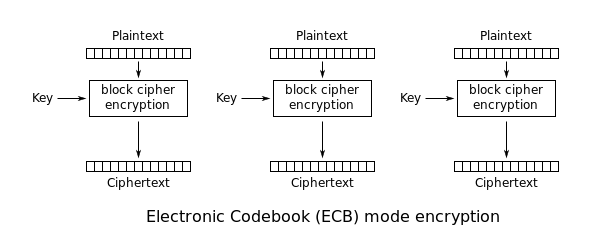
\includegraphics[width=0.499\textwidth]{images/block-ecb}}}
	\subfloat{{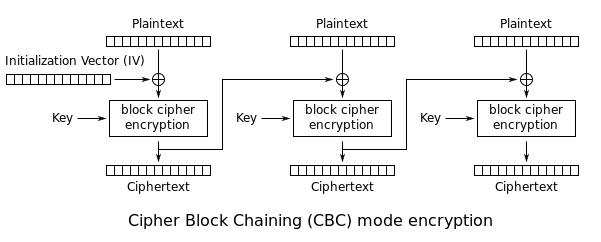
\includegraphics[width=0.499\textwidth]{images/block-cbc}}}
	\\
	\subfloat{{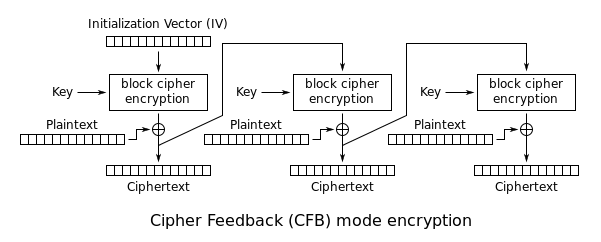
\includegraphics[width=0.499\textwidth]{images/block-cfb}}}
	\subfloat{{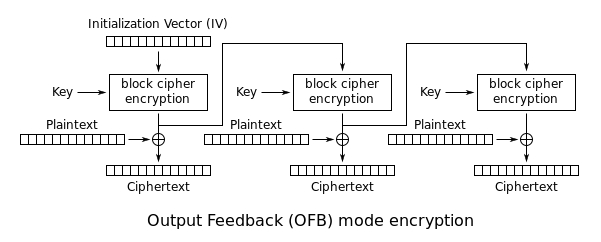
\includegraphics[width=0.499\textwidth]{images/block-ofb}}}
	\\
	\subfloat{{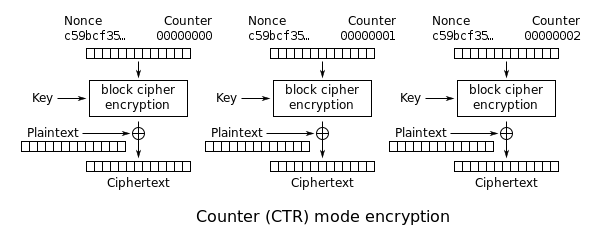
\includegraphics[width=0.499\textwidth]{images/block-ctr}}}

	\caption*{Schémata některých módů operací. Převzato z~\href{https://en.wikipedia.org/wiki/Block_cipher_mode_of_operation}{Block cipher mode of~operation}.}
\end{figure}

\subsection{\href{https://en.wikipedia.org/wiki/Data_Encryption_Standard}{DES}}

Jedna z~prvních globálně používaných blokových šifer. Využívá 56b klíče a~pracuje s~64b bloky v~šestnácti rundách. Využívá Feistelovo schéma (pro~\enquote{míchání} dvou 32b polovin bloku). Funkce $f$ se skládá z~expanze (32b půlblok na~48b), XOR s~rundovním klíčem (ten je získán pomocí \emph{Key scheduleru} různými bitovými posuny), S-boxu a P-boxu.

Není dostatečně bezpečný (brute-force útoky, diferenciální a~lineární kryptoanalýza). Poprvé zlomen 1997, v~roce 2016 zlomený během patnácti dnů na GTX 1080 Ti.

\subsubsection{3DES}

Také Triple DES, TDES. Využívá DES třikrát za~sebou za~účelem zvýšení jeho bezpečnosti. 3DES využívá tři 56b klíče a~\emph{ciphertext} je získán výpočtem $c = E_{K3}(D_{K2}(E_{K1}(m)))$%
\footnote{Šifrování prvním klíčem, dešifrování druhým a~šifrování třetím. 3DES totiž nabízí možnost použít i~dva klíče, kdy $K3=K1$.}%
. 3DES je náchylný na~\href{https://en.wikipedia.org/wiki/Meet-in-the-middle_attack}{\emph{Meet-in-the-Middle} útok} a~některé \emph{chosen-plaintext}/\emph{known-plaintext} útoky, OpenSSL ho neobsahuje od~roku 2016 a~NISTem byl prohlášen za~nedostatečně bezpečný v~roce 2017.

\subsection{\href{https://en.wikipedia.org/wiki/Advanced_Encryption_Standard}{Rijndael}}

Ke~konci 90. let bylo třeba vyměnit nedostatečně silné DES/3DES, Rijndael%
\footnote{Rijndael, holandská výslovnost [\textipa{"rEinda:l}]}
je vítězný kandidát pro~šifru AES, je rychlý na~hardware i~sofware. AES využívá klíče o~délce 128b/192b/256b a~128b bloky.

% Je tu ošklivé rozdělení "key addition" protože \underline neumí dělit řádky; bylo by nutné použít \uline z balíčku ulem
\textbf{Rundovní operace} (na~bloku 4x4B): \underline{substituce} (S-box): šestnáct bijektivních operací, v~software řešeno překladovou tabulkou, \underline{\emph{row shift}} (bajtová permutace): rotace \mbox{$i$-tého} řádku o~$i-1$ pozic doleva, \underline{\emph{column mix}} (lineární transformace): vynásobení matic, \underline{\emph{key}} \underline{\emph{addition}}: XOR s~rundovním klíčem. V~první rundě se provádí pouze přidání klíče, v~poslední pouze substituce, \emph{row shift} a~přidání klíče.

I~když existují útoky na~oslabené verze AES (nižší počet rund a~menší velikost klíčů), jde o~bezpečný protokol který je využitý v~TLS, OpenSSH a~většině ostatních současných protokolů.

\clearpage
\section{Asymetrické algoritmy -- RSA, Diffie-Hellman, ECDH systém a jejich využití pro digitální podpis.}

Problém diskrétního logaritmu%
\footnote{\emph{Discrete Logarithm Problem}, DLP}%
: $$c = m^n \Mod p$$ je pro velká čísla neřešitelné.

\subsection[RSA]{\href{https://en.wikipedia.org/wiki/RSA_(cryptosystem)}{RSA}}

Jde o~relativně pomalý algoritmus, proto se s~ním nešifrují přenášená data samotná, ale pouze klíče pro~symetrickou kryptografii.

\begin{table}[ht]
\begin{tabular}{ll}
Vygenerování privátních prvočísel & $p, q$ \\
Vypočítání privátního čísla & $\phi(n) = (p-1)(q-1)$ \\
Vypočítání veřejného čísla & $n = p \cdot q$ \\
Vypočítání veřejného klíče & $k_{\mathrm{pub}} \in [1, n], \mathrm{GCD}(k_{\mathrm{pub}}, \phi(n)) = 1$ \\
Vypočítání privátního klíče & $k_{\mathrm{priv}} = k_{\mathrm{pub}}^{-1} \Mod \phi(n)$ \\
\end{tabular}
\end{table}

Parametry $p, q$ by měly být podobně velké, i~když s~trochu rozdílnou velikostí (pro~ztížení útoků). Jejich společné faktory by měly být co nejmenší, pokud to prvočísla nejsou. Místo funkce $\phi$ se v~praxi používá Carmichaelovu funkci $\lambda$, protože $\phi$ může generovat čísla větší než je třeba.

\begin{table}[ht]
\begin{tabular}{ll}
šifrování & $c = m^{k_{\mathrm{pub}}} \Mod n$ \\
dešifrování & $m = c^{k_{\mathrm{priv}}} \Mod n$ \\
podepisování & $\mathrm{Sig}_m = m^{k_{\mathrm{priv}}} \Mod n$ \\
ověření & $\mathrm{Sig}_m^{k_{\mathrm{priv}}} \stackrel{?}{=} m \Mod n$ \\
\end{tabular}
\end{table}

\subsection[Diffie--Hellman výměna]{\href{https://en.wikipedia.org/wiki/Diffie-Hellman_key_exchange}{Diffie-Hellman výměna}}

Veřejnými prvky jsou prvočíslo $p$ (s~velikostí nad~2048b), prvočíslo $q$ (větší než~224b) a~generátor $z \in \mathbb{Z}_p^*$ velikosti $q$. Jde o~systém náchylný na~MitM, klíče nejsou nijak autentizované.

\begin{table}[ht]
\centering
\begin{tabular}{lcl}
Alice && Bob \\
$1 \le a \le p-2$ && $1 \le b \le p-2$ \\
$A = g^a \Mod p$ & $\stackrel{A}{\rightarrow}$ $\stackrel{B}{\leftarrow}$ & $B = g^b \Mod p$ \\
$k = B^a \Mod p$ && $k = A^b \Mod p$ \\
\end{tabular}
\caption*{Znázornění DH výměny.}
\end{table}

\subsection{Diffie--Hellman výměna nad~eliptickými křivkami}

Vlastnosti ECDH jsou totožné s~DH, DLP je pouze nahrazen jeho verzí nad~křivkami (ECDLP). Násobení na~eliptických křivkách je aplikováno jako opakované přičítání bodu. Asymetrické kryptosystémy nad~eliptickými křivkami nabízí stejnou bezpečnost při~mnohem kratší délce klíče (3072b DH $\approx$ 160b ECDH).

\begin{table}[ht]
\centering
\begin{tabular}{lcl}
Alice && Bob \\
$a$ && $b$ \\
$A = aP \Mod p$ & $\stackrel{A}{\rightarrow}$ $\stackrel{B}{\leftarrow}$ & $B = bP \Mod p$ \\
$k = aB \Mod p$ && $k = bA \Mod p$ \\
\end{tabular}
\caption*{Znázornění ECDH výměny.}
\end{table}

\subsection{Digitální podpisy}

RSA, ElGamal, DSA, ECDSA, ověření certifikátu, blockchain, PKCS\#1, X.509, \dots

\begin{center}
{\huge \dots} zde je třeba doplnit zbytek {\huge \dots} \\
(vlastně sám nevím co by tu přesně mělo být)
\end{center}

\clearpage
\section{Hašovací funkce -- vlastnosti, princip, použití, kolize, odolnost proti kolizím, příklady.}

Hashovací funkce slouží k~vyjádření reprezentace dat pomocí krátného řetězce. Jejími požadavky jsou \textbf{jednosměrnost} (z~hashe nelze získat původní data), \textbf{bezkoliznost} (vytvořit dva soubory se~stejným otiskem je velmi obtížné až~nemožné) a~\textbf{rychlost}.

Bezkoliznost prvního řádu (\emph{preimage resistance}) zabraňuje nalezení vzoru, bezkoliznost řádu druhého (\emph{second preimage resistance}) zabraňuje ke~zprávě $m_1$ nalézt $m_2$ takovou, aby platilo $h(m_1) = h(m_2)$.

\subsection{Konstrukce}

Jedním ze~způsobů je rozdělení na~$n$-bitové bloky, které jsou zpracovány XOR. Také je možné bloky řetězit: $h_i = E(m_i, h_{i-1})$, použít kompresní funkci ($h_i = f(m_i, h_{i-1})$). Před vstupem do~iteračního procesu se zarovnává poslední blok a~přidává se za~ním blok s~délkou zprávy (tzv. Damgard-Merklovo zesílení).

\subsection{Využití}

\textbf{Zkrácení zprávy} na~její otisk (pro~digitální podpisy), \textbf{autentizace}, zrychlení vyhledávání v~databázích, \textbf{hesla}, PRNG, \dots.


\subsection{Kolize}

Na~běžné současné hashovací funkce neexistují způsoby, jakými by šla původní data získat. Proto je nutné použít útok hrubou silou a~zkoušet jeden vstup za~druhým. % TODO Rainbow tables

Pro~kolizi prvního řádu (nalezení vzoru) je složitost $O(2^n)$, kde $n$ je délka původní zprávy. Pro~kolizi druhého řádu (nalezení kolizního souboru) je složitost $O(2^{n/2})$, což vyplývá z~tzv.~narozeninového paradoxu\footnote{
Stačí 23 náhodně vybraných lidí k~tomu, aby se s~pravděpodobností 50~\% našla dvojice, která má narozeniny ve~stejný den, u~skupiny třiceti lidí je pravděpodobnost 70~\%. Pravděpodobnost, že nikdo shodný datum narozenin mít nebude, je $\bar{p}(n) = \frac{365!}{365^n(365 - n)!}$. Obrácené tvrzení $p(n) = 1 - \bar{p}(n)$ překračuje hranici 0.5 pro~$n=23$.
Tomuto útoku se říká \href{https://en.wikipedia.org/wiki/Birthday_attack}{narozeninový útok} a narozeninovou hranici lze spočítat právě jako $2^{n/2}$.
}.

\subsection{Příklady}

128b \textbf{LM~Hash} je stará funkce využívaná v~OS Windows od~osmdesátých let do~verze Vista/Server 2008, v~nejnovějších systémech je možné ji zapnout. Dva (\emph{null-padded}) bloky po~sedmi bajtech jsou zašifrovány dvěma DES klíči a~spojeny zpět k~sobě. \\
128b \textbf{MD5} aplikuje 64 rund (XOR, bit shift, posouvání subbloků, \dots). Poprvé plně prolomena v~roce 2004, od~roku 2010 oficiálně prohlášena za~nedostatečně bezpečnou. Stále je možné ji používat jako kontrolu integrity. \\
224b/256b/384b/512b \textbf{SHA-2} se sada hashovacích funkcí využívajících XOR, \emph{bit shift} a~modulární sčítání. Existují útoky na~oslabené verze (méně rund), všechny funkce z~této rodiny jsou považovány za~bezpečné. \\
224b/256b/384b/512b \textbf{SHA-3} využívá algoritmus Keccak (\enquote{princip houby}) a~je součást SHA rodiny od~roku 2015.

\clearpage
\section{PKI -- certifikát X.509 struktura, certifikační autorita základní části, časová razítka, autorita časových razítek.}

\subsection{Public key infrastructure}

PKI neboli \emph{Public Key Infrastructure} je souhrn technických a~organizačních prostředků spojených s~vydáváním, správou, používáním a~odvoláváním platnosti kryptografických klíčů a~certifikátů. Zabraňuje použití falešné identity. Veřejný klíč je platný pouze v~případě potvrzení důvěryhodnou stranou (certifikační autoritou).

\subsection{X.509}
Struktura:
\begin{itemize}[noitemsep]
    \item verze (\texttt{0}: x.509 verze 1, \texttt{1}: x.509 verze 2, \texttt{2}: x.509 verze 3),
    \item sériové číslo,
    \item algoritmus použitý pro~podpis,
    \item vydavatel (identifikace certifikační autority dle x.500),
    \item platnost od--do,
    \item jméno a~adresa vlastníka,
    \item veřejný klíč,
    \item rozšíření certifikátu,
    \item digitální podpis certifikátu.
\end{itemize}

Certifikáty x.509 se ukládají ve~formátu PEM (\emph{Privacy Enhanced Mail}; hlavička a~ASCII formát v~base64), DER/BER (\emph{Distinguished Encoding Rules}, \emph{Basic Encoding Rules}; binární formát, při~jehož konverzi a~přidání hlavičky vznikne PEM) a ASN.1 (popis dat dobře čitelný lidmi).

\subsection{Certifikační autorita CA}

Základními částmi jsou třída 1, 2, 3.

V~\textbf{třídě 1} ručí CA pouze za~jednoznačnost certifikátu. Registrační autoritu takové CA je možné zjednodušit na~program neboli žadatel vyplní formulář serveru a~protokolem HTTPS jej odešle (stačí autentizace serveru a~klient je tedy anonymní).

\textbf{Třída 2} zahrnuje vše z~třídy 1 a~navíc kontroluje totožnost uživatele: k~zástupci registrační autority osobně dochází žadatelé. RA ověří totožnost uživatele a~odešle žádost CA. CA třídy 2 uchovává svůj soukromý klíč v~bezpečném hardwaru.

\textbf{Třída 3} zahrnuje vše co třída 2, ale certifikáty jsou určené pro~konkrétní aplikaci a~pro~nic jiného se nepoužívají. Př.: certifikát lze použít k přihlášení do nějaké aplikace ale email s ním nejde podepsat. Zde se soukromý klíč také uchovává v bezpečném hardwaru.

Další části CA jsou registrační autority (RA), online RA, IVR nebo telefonní záznamník, adresářové služby, DVCS server, timestamp server a~zúčtovací systém.

\textbf{Registrační autorita} má na~starosti žádosti o~certifikáty. Ověří totožnost uživatele, verifikuje žádost o~certifikát a~předá ho certifikační autoritě. CA ověří údaje z~žádosti uživatele a~údaje doplněné RA a~vydá nebo nevydá příslušný certifikát.
 
\textbf{Online RA} přijímá žádosti online cestou a~lze zažádat o:
\begin{itemize}
    \item obnovení certifikátu v~době platnosti starého,
    \item vydání nového certifikátu na~základě jednorázového hesla pro vydání~ certifikátu,
    \item další certifikáty, žádost se podepisuje platným certifikátem,
    \item soukromý šifrovací klíč, který je archivován na~CA,
    \item odvolání certifikátu,
    \item CRL (\emph{Certificate revocation list}, seznam odvolaných certifikátů) nebo jiný certifikát vydaný CA.
\end{itemize}

\textbf{IVR nebo telefonní záznamník} slouží k~odvolání certifikátu telefonem (jinou cestou). Pro~odvolání musí proběhnout autentizace jednorázovým heslem.

\textbf{Adresářové služby} nabízejí informace o~uživatelích, které si uživatelé o~sobě přejí publikovat (vydané certifikáty).

\textbf{DVCS server} poskytuje informace o~platnosti certifikátu, listin a~dále může poskytovat časová razítka protokolem DVCSP.

\textbf{Timestamp server} je speciální server poskytující pouze časová razítka a~nemusí mít přístup do~archívu CA.

\textbf{Zúčtovací systém} má za~cíl vystavit fakturu za~poskytnuté služby uživateli.

\textbf{Důležitá aktiva CA}, která se musí maximálně chránit jsou soukromý klíč CA, databázi uživatelů CA (CA nesmí vydat dvěma uživatelům stejný certifikát a~obsahuje osobní údaje), archiv soukromých šifrovacích klíčů uživatelů (pokud CA poskytuje), archiv listin uložených na~CA a~archiv vydaných certifikátů a~CRL.
\begin{center}
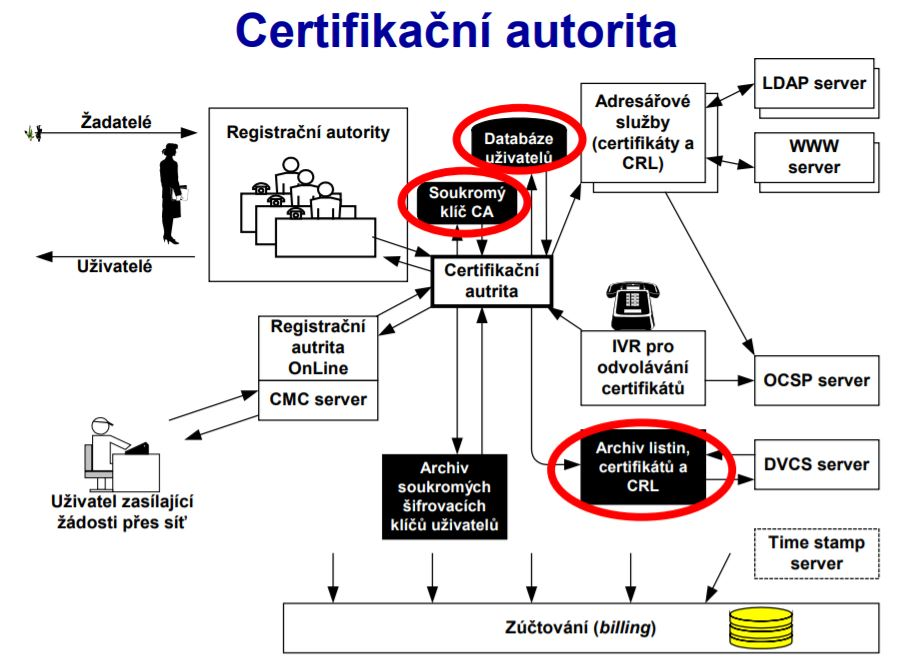
\includegraphics[scale=0.5]{images/CA.jpg}
\end{center}

\subsection{Časová razítka (time stamp)}

Časová razítka jsou elektronický ekvivalent časového určení a místa vlastního podpisu na listině. Řeší možné problémy vzniklé problémy odvoláním certifikátu. Zajišťuje především důkaz o existenci dokumentu v daném čase. Využívá se k poskytovaní elektronických notářských služeb a zajištění dlouhodobé archivace elektronicky podepsaných dokumentů. Časové razítko svazuje hash dokumentu s časem.

\noindent Struktura obsahuje:
\begin{itemize}[noitemsep]
    \item Jméno vydavatele (jméno autority pro vydávání časových razítek (TSA)).
    \item Jedinečné sériové číslo razítka.
    \item Hash dokumentu a čas.
\end{itemize}

\subsection{Autorita časových razítek (TSA)}

TSA musí podepisovat každé časové razítko privátnín klíčem vyhrazeným pouze k tomuto účelu. TSA musí být napojena bezpečným způsobem a v pravidelných časových intervalech synchronizována proti nejlépe třem na sobě nezávislým zdrojům. TSA využívají mezinárodní standard coordinated universal time UTC.

\noindent Požadavkům na zdroj času lze dosáhnout využitím PKI, zajišťující důvěrnost, integritu, neodmítnutelnost a autenticitu při časové synchronizaci. Požadavky na zdroj času jsou:

\begin{itemize}[noitemsep]
    \item Musí pocházet z oficiálního důvěryhodného zdroje.
    \item Čas nesmí být možné cestou změnit.
    \item Vždy musí být možné zpětně dohledat zdroj času (celou hierarchii časových serverů)
\end{itemize}

\subsection{Vydání časového razítka}

Uživatel zažádá pomocí klientské aplikace. Klient vytvoří a odešle žádost o časoví razítko ve standardizovaném formátu. Žádost je datová struktura obsahující hash dokumentu. TSA v případě kladné odpovědi odesílá odpověď obsahující časové razítko.

\begin{center}
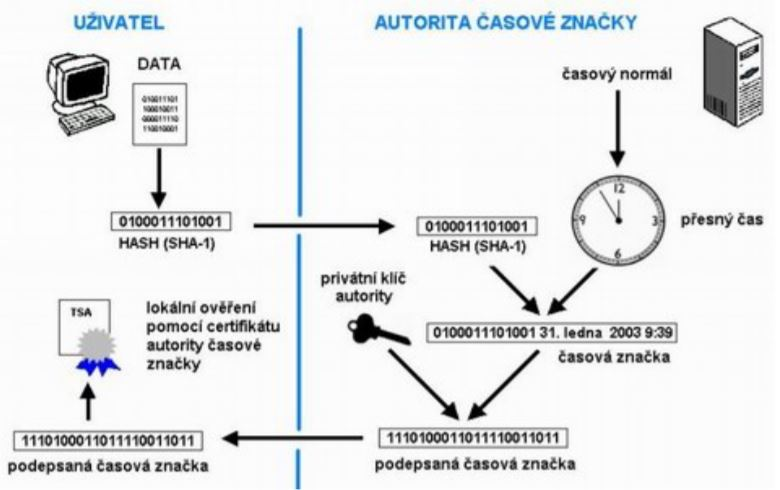
\includegraphics[scale=0.7]{images/Timestamp.jpg}
\end{center}

\clearpage
\section{Generování náhodných čísel -- kryptografické generátory, požadavky, použití, princip, testování generátorů.}

Hlavními požadavky na~RNG jsou \textbf{rovnoměrné rozložení} (hodnoty jsou generovány se~stejnou pravděpodobností), \textbf{nezávislost hodnot} (neexistuje korelace mezi nimi), \textbf{nepredikovatelnost} (na~základě znalosti čísla nebo řady čísel nelze předpovědět následující, tzv. \emph{next-bit test}) a~často také \textbf{rychlé generování} nebo odolnost vůči kompromitaci (při~zjištění vnitřního stavu nelze zpětně rekonstruovat dosavadní vygenerovanou posloupnost, tzv. \emph{state compromise}). \emph{Next-bit} ochrana a~zábrana kompromitace jsou požadavky kryptograficky bezpečných generátorů.

K~vytvoření dostatečného počtu (pseudo)náhodných čísel je nutná dostatečná entropie (míra náhodnosti/nepředvídatelnosti). Když útočník následující hodnotu zná, entropie je nulová. Lze ji vyjádřit jako $H(X) = - \sum_{i=1}^{n} p_i \log_2 p_i$ kde $X$ je generovaná hodnota a~$p_1, \dots, p_n$ jsou pravděpodobnosti hodnot $X_1, \dots, X_n$ které je generátor schopen vygenerovat.

\subsection{Typy generátorů}

\subsubsection*{Fyzikální generátory (TRNG)}

Teoreticky jsou nedeterministické, nejsou ale známy přesné parametry, kterými by se daly popsat a~modelovat. Zaručují maximální bezpečnost a~neopakovatelnost. Nevýhodou je pomalé generování či~problematická technická realizace. Příklady: radioaktivní rozpad, tepelný šum, kvantové generátory.

\subsubsection*{Algoritmické generátory (PRNG)}

Posloupnost náhodná není, pokud útočníkovi jsou známy některé parametry generátoru. Výhodami je rychlost, nízká odchylka od~poměru 1:1 nebo snadná realizace. Nevýhodami jsou bezpečnost či~periodicita. Příklady: čas, teplota HW komponent, šum na~\emph{low-level} sběrnicích (USB, pohyb myši), pohyb HDD.

\subsubsection*{Smíšené generátory}

TRNG z~fyzikálního generátoru se~spojí s~PRNG výstupem pomocí XOR.

\subsection{Příklady realizace PRNG}

\textbf{Bloková šifra v~režimu čítače}: náhodně se zvolí klíč a~počáteční hodnota $i$; zvoleným klíčem se šifrují hodnoty $i, i+1, \dots$ -- perioda u~$n$-bitové šifry je $2^n$. \\
\textbf{Hashovací funkce aplikovaná na~čítač}: hashuje se $i, i+1, \dots$. \\
\textbf{Proudové šifry}: viz otázku \ref{question-4}.

\subsection{Konkrétní příklady}

\textbf{\href{https://en.wikipedia.org/wiki/Blum_Blum_Shub}{Blum-Blum-Shub PRNG}} má formu $x_{n+1} = x_n^2 \Mod M$ (kde $M = pq$ je násobek dvou velkých prvočísel), výstup je~získán pomocí bitové parity výsledku, nebo z~jednoho či více nejméně významých bitů. Byl navrhnut v~roce 1986. \emph{Seed} by mělo být číslo nesoudělné s~$M$, s~vyloučením $\{0, 1\}$.

\textbf{Linuxový PRNG} sbírá události (myš, klávesnice, HDD, síť, \emph{system interrupts}, systémový čas). Zdroj \texttt{/dev/random} je blokující (při~nedostatku entropie se~čeká), na~rozdíl od~\texttt{/dev/urandom} (\emph{unblocked random}), kdy je vráceno \enquote{méně náhodné číslo}.

\textbf{EGD (Entropy Gathering Daemon)} využívají některé linuxové programy (OpenSSL, GPG, Apache HTTP) pokud není dostatečné množství náhodných bitů v~\texttt{/dev/random}. Entropii sbírá ve~stavu CPU, IO nebo sítě.

\subsection{Testování}

K~ověření vlastností PRNG se využívají statistické testy. Odhalí nekvalitní PRNG, ale neprokážou kvalitní PRNG. Testy vrací $p$-hodnotu, která vyjadřuje sílu důkazů proti nulové hypotéze (\enquote{Testovaná posloupnost je náhodná.}). Pokud $p$-hodnota překročí určitou mez, nulovou hypotézu považujeme za~neplatnou.

\textbf{Frekvenční test}: Obsahuje testovaná posloupnost bitů přibližně stejný počet nul a~jedniček? \textbf{Runs test}: Je počet a~délka řetězců po~sobě jdoucích stejných bitů na~úrovni náhodné posloupnosti? \textbf{Test hodností matic}, \textbf{spektrální test}.


\clearpage
\section{Bezpečnostní architektura RM OSI -- služby bezpečnosti, mechanizmy bezpečnosti, útoky na bezpečnost, příklady implementace bezpečnostních mechanizmů v jednotlivých vrstvách.}

\subsection{Architektura bezpečnosti v RM OSI}

K zabezpečení se používá doporučení ITU-T X.800, ISO 7498-2 ISO/OSI Security Architecture. Obsahuje mechanismy bezpečnosti (security mechanism), útoky na bezpečnost (security attacks) a službu bezpečnosti (security services), kde jsou definované postupy pro zabezpečení informačních systémů.

\subsection{Implementace bezpečnostních funkcí ve vrstvách RM OSI}

Pro implementaci jsou nejvhodnější vrstvy 7. (aplikační protokoly), 4. (transport dat) a 3. (směrovaní). Bezpečnostní mechanismy jsou zabudovány do aplikačních programů a operačních systémů (7. a 4. vrstva)  a propojovacích zařízení (3. vrstva) ale existují i způsoby zabezpečení, které využívají další vrstvy.

\subsection{Služby bezpečnosti}

Služba bezpečnosti je realizovaná protokolem příslušné vrstvy. Existuje 5 kategorií služeb, kterými jsou autentizace (authentication), řízení přístupu (access control), zabezpečení důvěrnosti dat (data confidentiality), zabezpečení integrity dat (data integrity) a ochrana proti odmítnutí původní zprávy (non-repudiation).

\textbf{Autentizace} je proces ověřovaní identity uživatele (entity). Existuje autentizace uživatelů (peer entity authentication), které nezabraňují útoky zopakováním zpráv. Dále existuje autentizace zdroje dat (data origin authentication), která provádí autentizaci všech dat a zabraňuje útokům zopakováním zpráv.

\textbf{Řízení přístupu}: kontrola přístupu (možnost povolit nebo odepřít použití určitého zdroje určitému subjektu, řízení přístupu k materiálním, logickým, nebo digitálním zdrojům \textbf{neplést si s autorizací}). Umožňuje přístup  do systému k službám a dalším. Chrání před neautorizovaným přístupem, kde se nejčastěji nachází v aplikaci nebo OS.

\textbf{Zabezpečení důvěrnosti dat} je ochrana obsahu dat, ochrana toku dat při přenosu proti analýze (zjištění odesílatele, adresáta, \dots). 

\noindent Obsahuje služby pro:
\begin{itemize}[noitemsep]
    \item Důvěrnost přenosu zprávy.
    \item Důvěrnost spojení (ochrana důvěrnosti v rámci navázaného spojení).
    \item Důvěrnost toku dat (chrání informace na zálkadě atributů toku dat).
    \item Selektivní důvěrnosti (ochrana pouze určených částí informace).
\end{itemize}

\textbf{Zabezpečení integrity dat} se zabývá zabezpečením proti neautorizované modifikaci (autorizace je přiřazení oprávnění pro práci v systému, specifikují se činnosti). Spadají sem služby integrity přenosu zpráv (ochrana integrity všech přenášených zpráv), služba integrity spojení (ochrana přenosů v rámci určitého navázaného spojení) a služby selektivní integrity spojení a selektivní integrity zpráv.
Integritu rozdělujeme na slabou a silnou.

\noindent \textbf{Slabá integrita} slouží pro objevování útoků (modifikace zprávy šumem, náhodná změna pořadí paketů, náhodná duplicita \dots) pomocí aplikací kontrolních součtů, CRC, pořadová čísla paketů atd.

\noindent \textbf{Silná integrita} zabezpečuje proti úmyslným, aktivním útokům (subjektivní útoky) jako jsou podvržení zprávy, úmyslné pozměnění zprávy. Celkově silnou integritu tvoří prostředky slabé integrity a kryptografické prostředky


\textbf{Ochrana proti odmítnutí původu zprávy} zajišťuje důkaz o původnosti dat, prokazuje původ (příjemce, odesílatel) a prokazuje doručení (odesílaní, přijetí).

\vspace{0,5cm}
Celkově by měla být zajištěna autentizace (vím s kým komunikuji) a nepopiratelnost (vím s kým komunikuji a lze to dokázat).

\subsection{Mechanizmy bezpečnosti}

Mechanizmy bezpečnosti jsou šifrování, digitální podpis, řízení přístupu, integrita dat, výměna autentizační informace, padding (výplň), řízení směrovaní a ověření třetím subjektem.

\subsection{Útoky na bezpečnost -- model hrozeb}
\begin{multicols}{2}
\noindent \textbf{Destruction} (útok na dostupnost) zničení dat či síťových zdrojů.

\noindent \textbf{Corruption} (útok na integritu) neautorizovaná modifikace aktiv nebo dat.

\noindent \textbf{Removal} (útok na dostupnost) krádež, odebrání či ztráta informací nebo jiných zdrojů.

\noindent \textbf{Disclosure} (útok na důvěrnost) neautorizovaný přístup k aktivům nebo datům.

\noindent \textbf{Interruption} (útok na dostupnost) přerušení služeb, spojení začně být nepoužitelné.

\begin{center}
    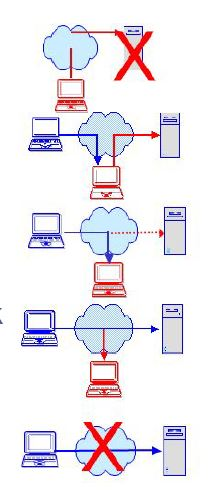
\includegraphics[scale = 0.6]{images/threatModel.JPG}
\end{center}
\end{multicols}

\subsection{Příklady implementace}

Na síťové vrstvě se o bezpečnost stará hlavně IPsec. Zajišťuje důvěrnost a integritu přenášených dat. O integritu se stará autentizační hlavička IP datagramu. Důvěrnost se zajišťuje pomocí mechanismu zapouzdření.

Na transportní vrstvě je bezpečnost zajištěna pomocí TLS (SSL bylo znehodnoceno v 2015) protokolu pro protokoly na aplikační vrstvě. Zajišťuje autentizaci mezi serverem a klientem, šifruje se spojení. Tímto zajišťuje autentizaci a důvěrnost.

Na aplikační vrstvě několik protokolů jako HTTPS, SSH a další. HTTPS zajišťuje důvěrnost, autentizaci a integritu. SSH zajišťuje autentizaci, integritu a důvěrnost přenášených dat.